\documentclass[a4paper, oneside, final]{memoir}
\usepackage[T1]{fontenc}
\usepackage[utf8]{inputenc}
\usepackage[british]{babel}
\usepackage{amsmath}
\usepackage{amsthm}
\usepackage{ifthen}
\usepackage{verbatim}
\usepackage{pdfpages}

% bedre orddeling Gør at der som minimum skal blive to tegn på linien ved
% orddeling og minimum flyttes to tegn ned på næste linie. Desværre er værdien
% anvendt af babel »12«, hvilket kan give orddelingen »h-vor«.
\renewcommand{\britishhyphenmins}{22} 

% Fix of fancyref to work with memoir. Makes references look
% nice. Redefines memoir \fref and \Fref to \refer and \Refer.
% \usepackage{refer}             %
% As we dont really have any use for \fref and \Fref we just undefine what
% memoir defined them as, so fancyref can define what it wants.
\let\fref\undefined
\let\Fref\undefined
\usepackage{fancyref} % Better reference. 

\usepackage{pdflscape} % Gør landscape-environmentet tilgængeligt
\usepackage{fixme}     % Indsæt "fixme" noter i drafts.
\usepackage{hyperref}  % Indsæter links (interne og eksterne) i PDF

\usepackage[format=hang]{caption,subfig}
\usepackage{graphicx}
\usepackage{stmaryrd}
\usepackage{amssymb}
\usepackage{listings}
\usepackage{ulem} % \sout - strike-through
\usepackage{tikz}

\renewcommand{\ttdefault}{txtt} % Bedre typewriter font
% \usepackage[sc]{mathpazo}     % Palatino font
\renewcommand{\rmdefault}{garamond} % Garamond
%\usepackage[garamond]{mathdesign}

% \overfullrule=5pt
% \setsecnumdepth{part}
\setcounter{secnumdepth}{1} % Sæt overskriftsnummereringsdybde. Disable = -1.
\setlength{\parskip}{0.25in}

\title{Statistical Methods for Machine Learning\\Case 1}

\author{Troels Henriksen (athas@sigkill.dk) \\ Daniel Fairchild}

\date{\today}
\pagestyle{plain}

\newcommand{\nfrac}[2]{\frac{\displaystyle{#1}}{\displaystyle{#2}}}

\begin{document}

\maketitle

We have never used R before, so for the novelty, that is the language
we have decided to use for this assignment.

\section*{Question 1.1}

The following plot has been produced through straightforward use of
the \texttt{dnorm} function and plotting facilities in R.  A thousand
sample points have been used.  The code for this question is in the
file \texttt{question11.R}.

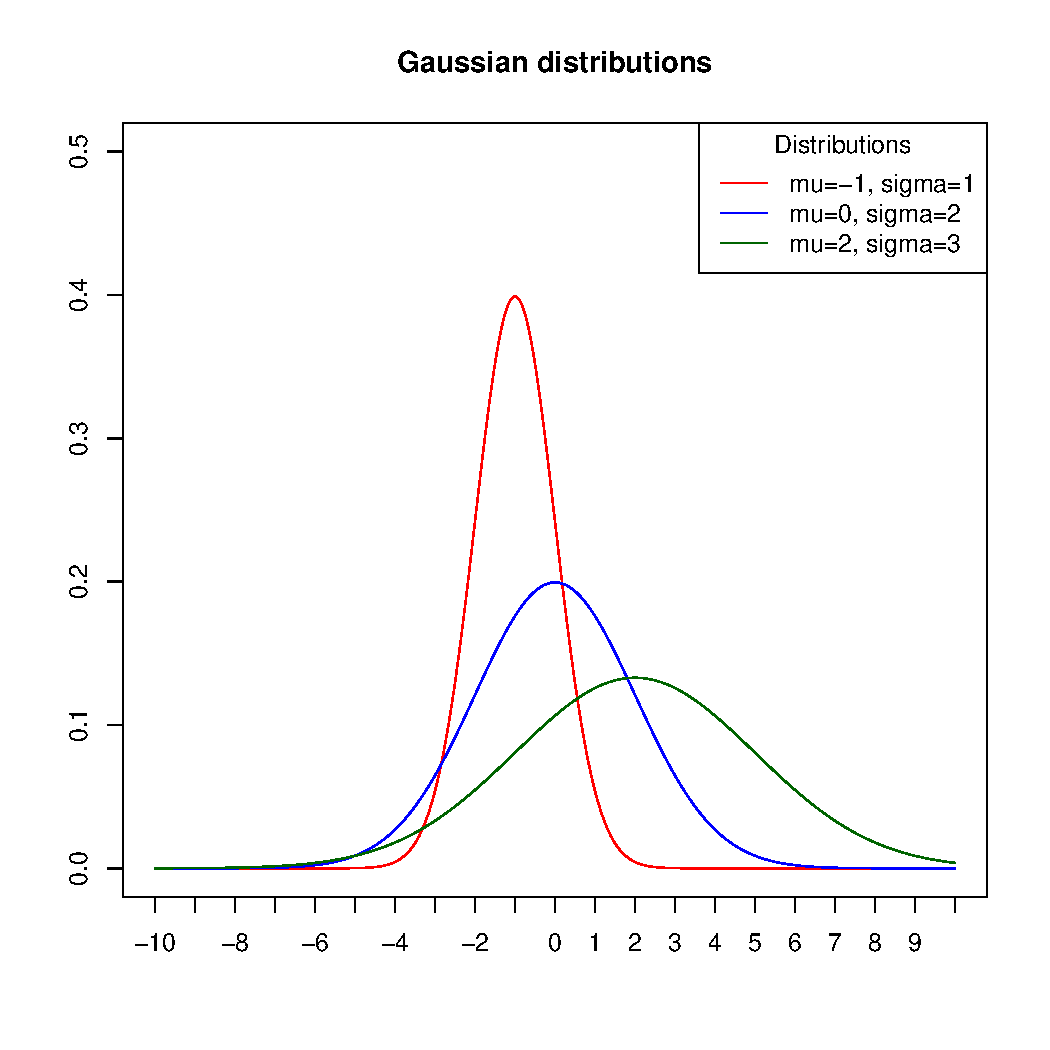
\includegraphics[width=10cm]{img/question11-plot.eps}

\section*{Question 1.2}

The matrix
\[
M=\left[\begin{matrix}
  x_{1,1}&\cdots&x_{1,m}\\\vdots&\ddots&\vdots\\x_{n,1}&\cdots&x_{n,m} \end{matrix}\right]
\]
is \textit{positive definite} if for any nonzero real-entried vector
\[
V=\left[\begin{matrix} y_1 \\ \vdots \\ y_m \end{matrix}\right]
\]
we have
\[
V^TMV > 0.
\]

$M$ is \textit{symmetric} if $M^T=M$.

$M$ is \textit{square} if $m=n$.

An eigenvalue $\lambda$ is positive if $\lambda > 0$.

\section*{Question 1.3}

The code for this question is in the file \texttt{question131415.R}.

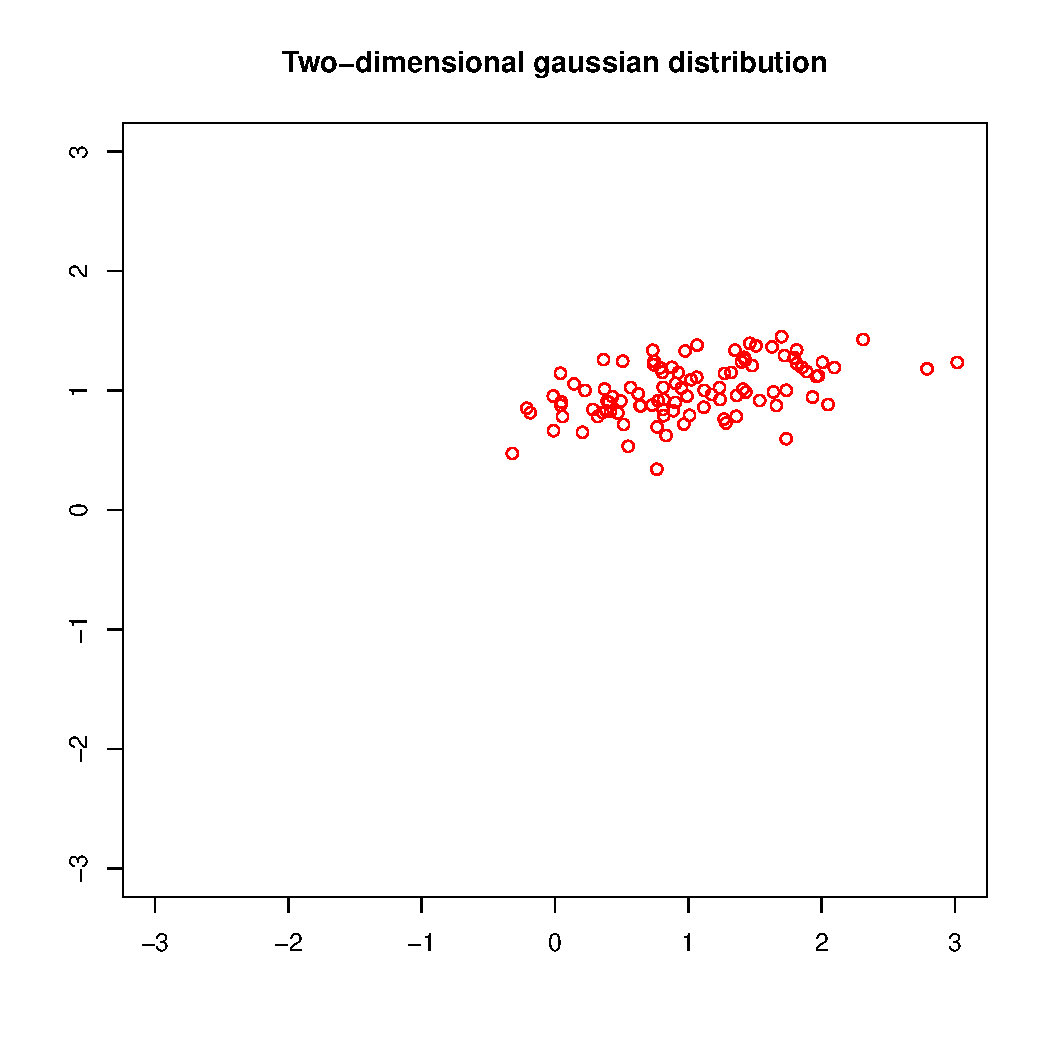
\includegraphics[width=10cm]{img/question13-plot.eps}

\section*{Question 1.4}

The code for this question is in the file \texttt{question131415.R}

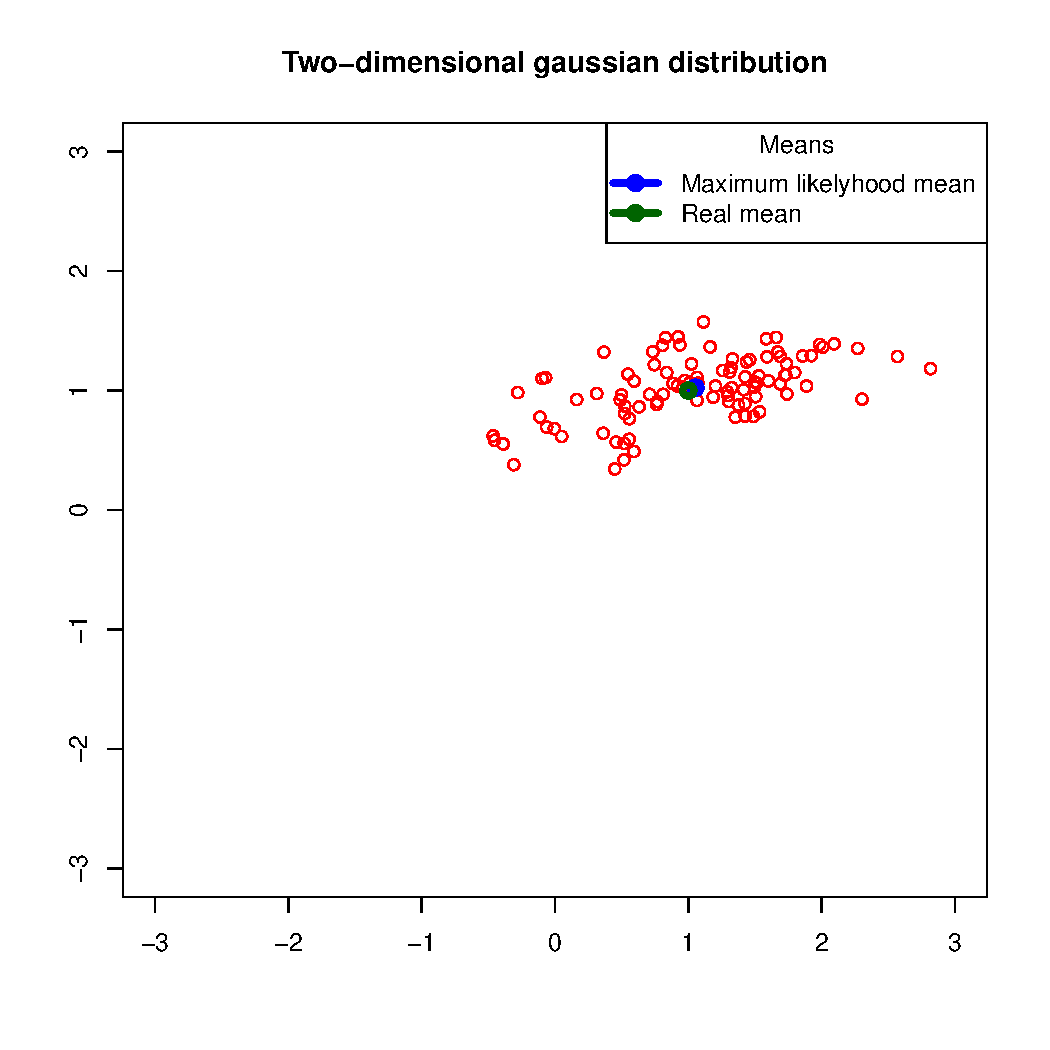
\includegraphics[width=10cm]{img/question14-plot.eps}

On a particular sampling the following sample covariance was observed
\[
\left[\begin{matrix}0.4995721&0.12549518\\0.1254952&0.07623185\end{matrix}\right]
\]
along with the sample mean
\[
\left[\begin{matrix}0.9653615\\0.9419024\end{matrix}\right]
\]

The Euclidian distance from the sample mean to the real mean is
\[
\sqrt{(0.9653615-1)^2+(0.9419024-1)^2}=0.06764
\]

This deviation could be due to rounding errors either in generating
the samples, or in computing the sample mean.  Another possibility is
sheer randomness.

\section*{Question 1.5}

The code for this question is in the file \texttt{question131415.R}.\\
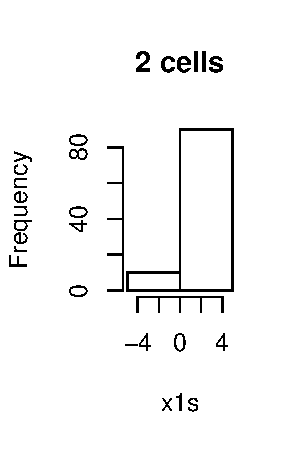
\includegraphics{img/question15-plot-1-a.eps}
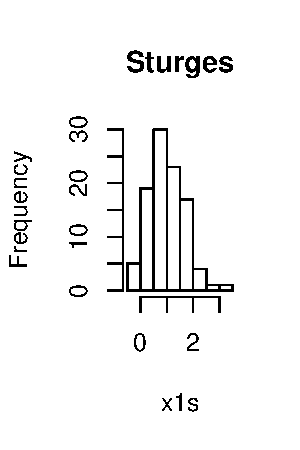
\includegraphics{img/question15-plot-1-b.eps}
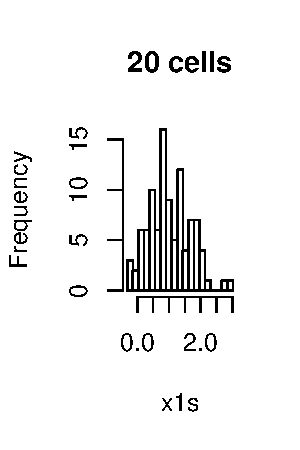
\includegraphics{img/question15-plot-1-c.eps}
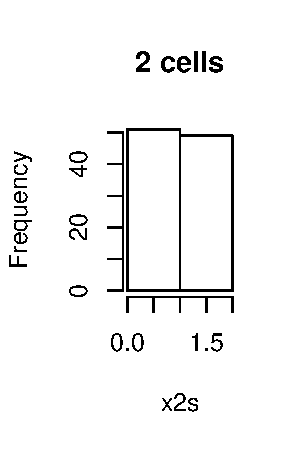
\includegraphics{img/question15-plot-2-a.eps}
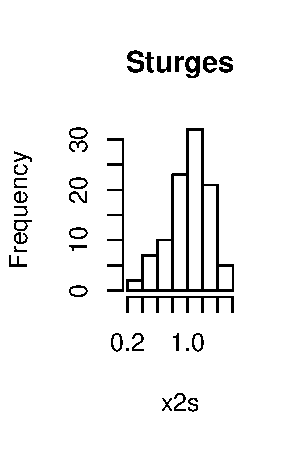
\includegraphics{img/question15-plot-2-b.eps}
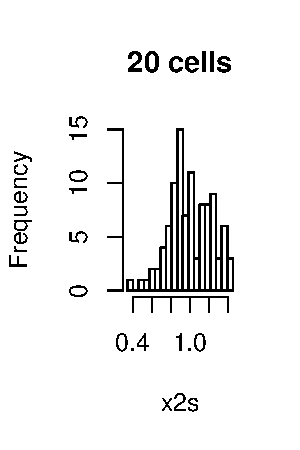
\includegraphics{img/question15-plot-2-c.eps}

As the bin width decreases, the random variation in the data results
in new local maximums that make the distribution appear more jagged
than it really is.

There is no best method to select bin widths, as the.  A common
method is Sturges' formula, where the $n$ data points are divided into
$\lceil\log_2n+1 \rceil$ bins.

\section*{Question 1.6}

The histogram is plotted with respect to density, rather than
frequency, so it can be easily compared to the density curve.  As can
be seen, the histogram with six bars fits the analytical curve well.

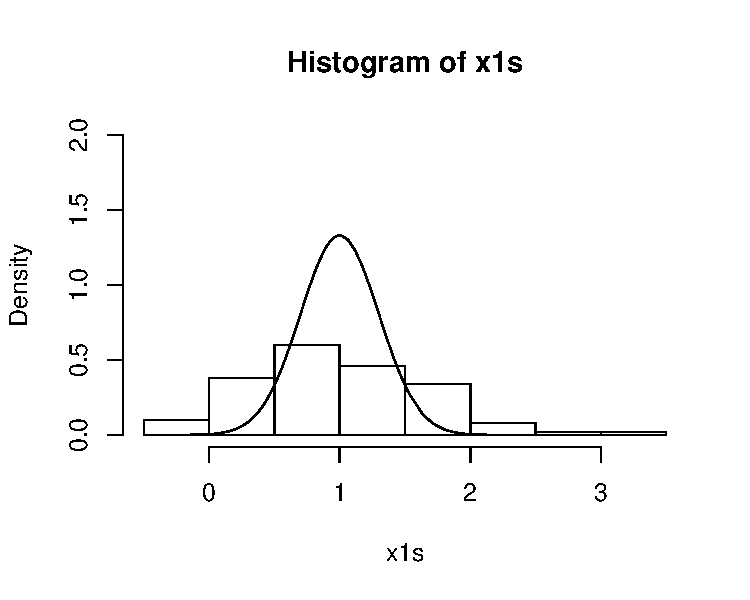
\includegraphics{img/question16-plot-analytical.eps}

The marginal distribution has the following analytical expression.

\begin{align*}
  p(x_1) &= \mathcal{N}(x_1|\mu_1,\Sigma_{1,1}) & \text{By CB (2.98)}\\
  &=
  \frac{1}{(2\pi\sigma_{1,1}^2)^{1/2}}\exp\left({-\frac{1}{2\sigma_{1,1}^2}(x_1-\mu_1)^2}\right)
  & \text{Substituting definition} \\
  &=
  \frac{1}{(2\pi\cdot 0.2^2)^{1/2}}\exp\left({-\frac{1}{2\cdot0.2^2}(x_1-1)^2}\right)
  & \text{Substituting $\sigma_{1,1}=0.2,\mu_1=1$}
\end{align*}

\section*{Question 1.7}

\includegraphics{img/question17-plot-100.eps}
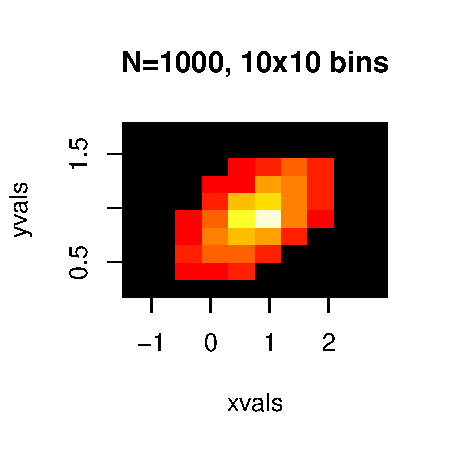
\includegraphics{img/question17-plot-1000-10x10.eps}
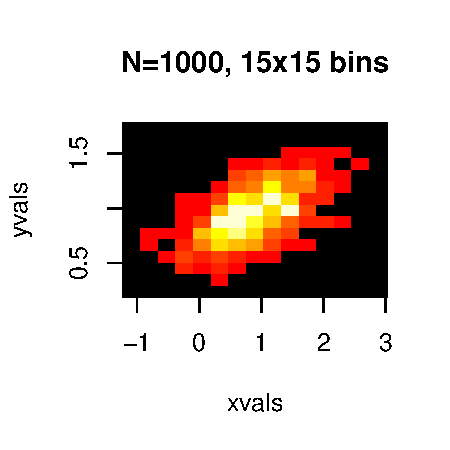
\includegraphics{img/question17-plot-1000-15x15.eps}
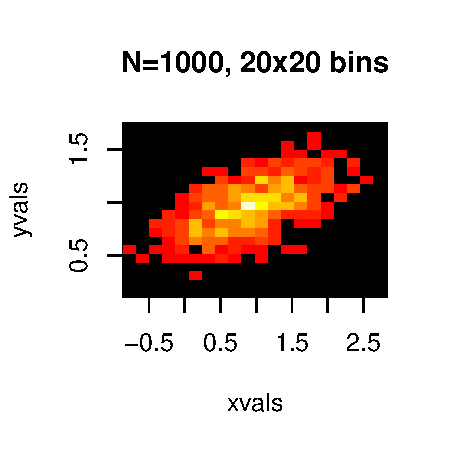
\includegraphics{img/question17-plot-1000-20x20.eps}
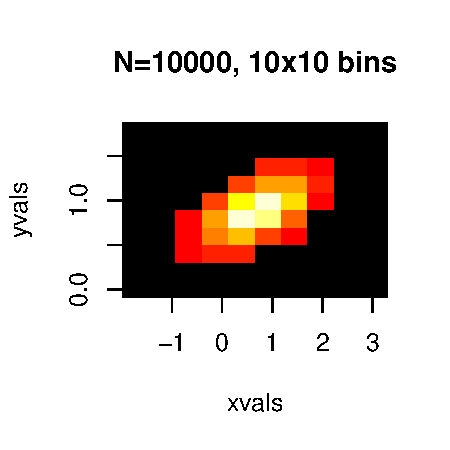
\includegraphics{img/question17-plot-10000.eps}

\section*{Question 1.8}


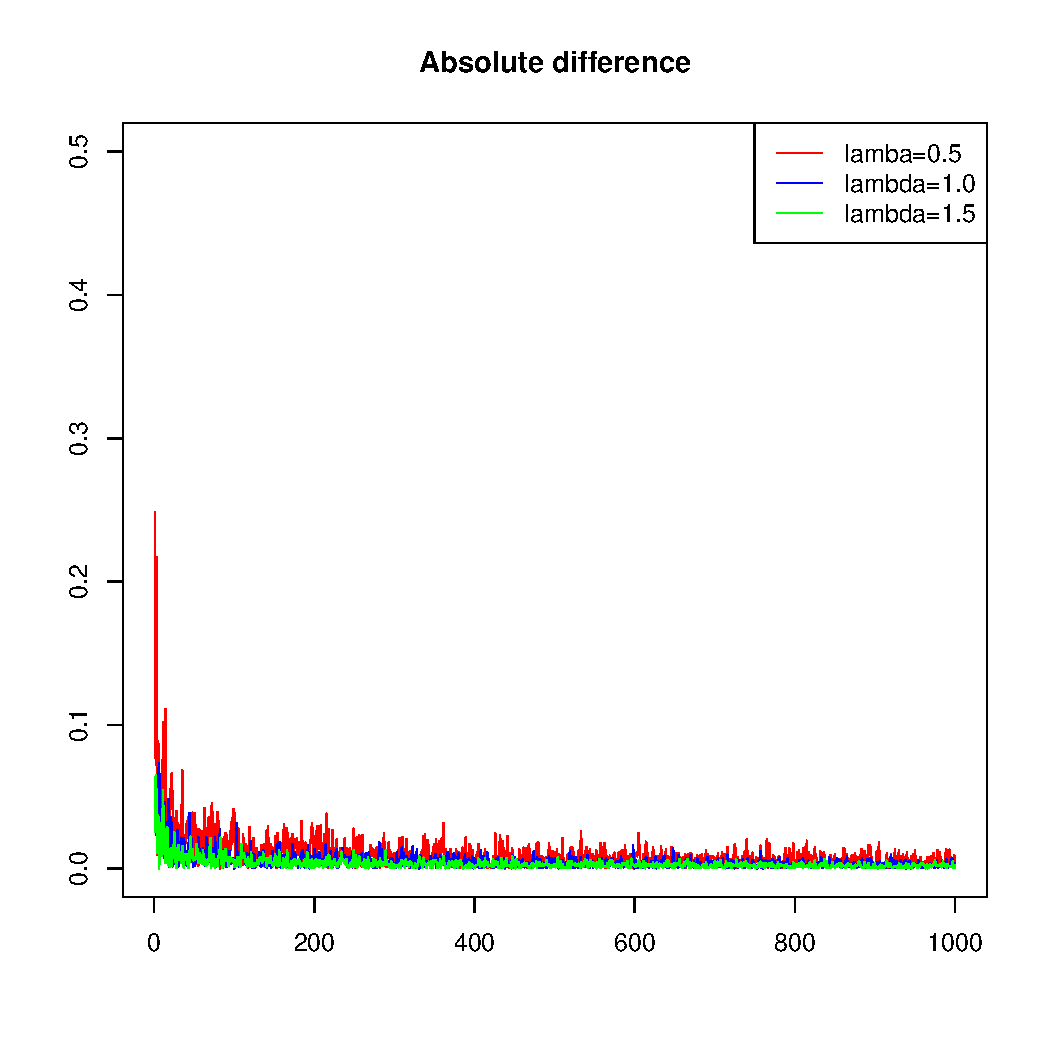
\includegraphics[width=10cm]{img/question18-plot-1.eps}

\end{document}
